%==================================================================%
% Author : Pando Muñoz, Manuel                                     %
%          Sánchez Barreiro, Pablo                                 %
% Version: 1.0, 30/03/2011                                         %
%                                                                  %
% Memoria del Proyecto Fin de Carrera                              %
% Archivo raíz para el capítulo de la arquitectura del sistema     %
%==================================================================%


\chapterheader{Arquitectura y diseño}{Definición Arquitectónica y Diseño Software}
\label{chap:arquitectura}

En el presente capítulo se presentan, mediante diagramas UML, la arquitectura física del sistema, los módulos y las comunicaciones entre ellos existentes en el sistema, y el funcionamiento del mismo.

 \todo{finalizar breve introducción}

\chaptertoc

\section{Arquitectura física del Sistema}
\label{sec:arquitectura:arqFisica}

En esta sección se describe la arquitectura física del sistema mediante un diagrama de despliegue.
\begin{figure}
    \centering
    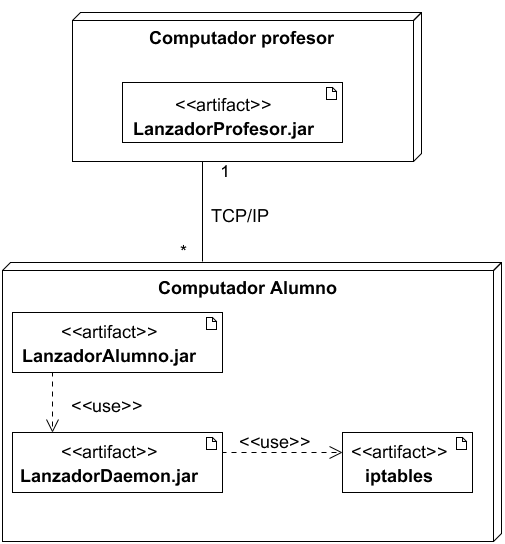
\includegraphics[width=\linewidth]{arquitectura/despliegueSistema2}
    \caption{Diagrama de despliegue del sistema}
    \label{fig:arquitectura:despliegueSistema}
\end{figure}
\newline


\lq\lq LanzadorProfesor.jar\rq\rq contiene lo necesario para mostrar la interfaz de usuario en la aplicación del profesor, así como la lógica de manejo de eventos y comunicación con las aplicaciones de los alumnos.

\lq\lq LanzadorAlumno.jar\rq\rq contiene las funciones para mostrar la interfaz de usuario de la aplicación del alumno, el manejo de eventos producidos por su uso y la lógica de comunicación con la aplicación del profesor y el demonio local.

\lq\lq LanzadorDaemon.jar\rq\rq contiene la lógica de comunicación con la aplicación del alumno y lo necesario para interactuar con iptables.

\lq\lq iptables\rq\rq es parte del núcleo del sistema Linux sobre el que se ejecutará la aplicación.

Cómo se puede puede observar, sólo se permite la existencia de una aplicación en el computador del profesor, a la que se conectan mediante TCP/IP un número indefinido de aplicaciones alumno, lógico, ya que en cada prueba suele haber varios los alumnos realizándola y uno el número de profesores.
\newline

A su vez, la aplicación del alumno interactúa con un único demonio del sistema.


\section{Diseño Software}
\label{sec:arquitectura:diseno}

En está sección se muestra un diagrama de actividad que resume las posibles interacciones que tanto el alumno como el profesor realizan con sus respectivas aplicaciones durante el trascurso normal de una prueba y un diagrama de estados para clarificar la aplicación del alumno.
\newline


\begin{figure}
    \centering
    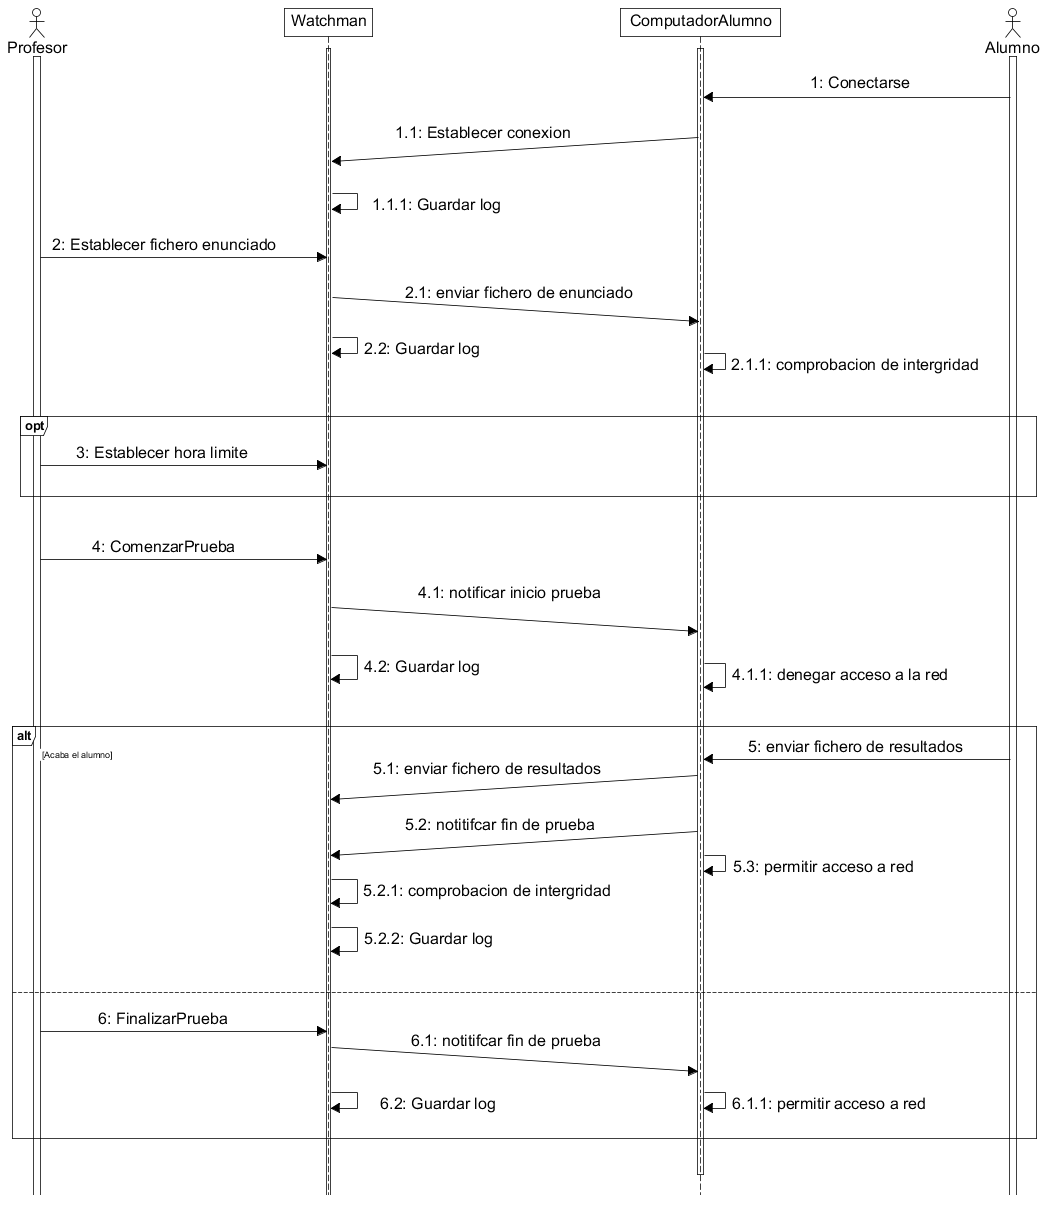
\includegraphics[width=\linewidth]{arquitectura/actividadSistema3}
    \caption{Diagrama de actividad del sistema}
    \label{fig:arquitectura:actividadSistema}
\end{figure}


Vemos en la figura \ref{fig:arquitectura:actividadSistema} que se siguen los pasos descritos en la sección \ref{sec:planificacion:descFuncional}



\begin{figure}
    \centering
    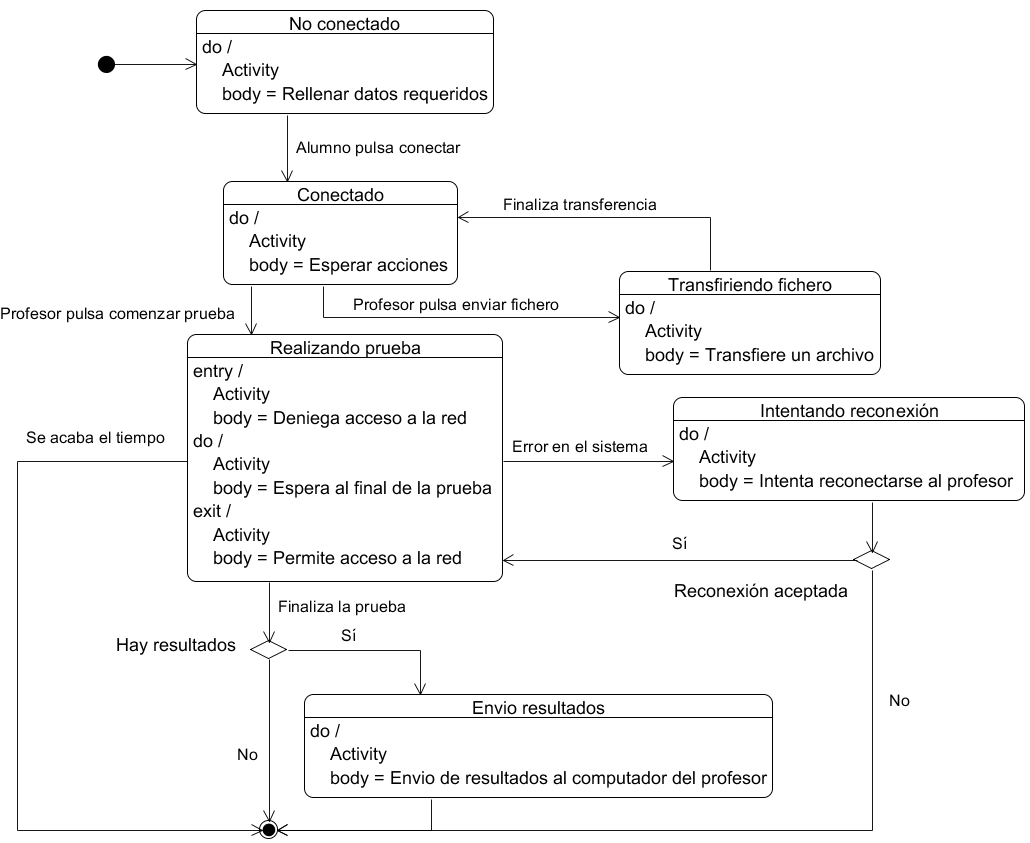
\includegraphics[width=\linewidth]{arquitectura/estadosAlumno2}
    \caption{Diagrama de estados de la aplicación del alumno}
    \label{fig:arquitectura:estadosAlumno}
\end{figure}


En la figura \ref{fig:arquitectura:estadosAlumno} se describen los estados por los que puede pasar la aplicación del alumno. Se corresponden directamente con el estado en que se encuentra la prueba.


\section{Seguridad del software}
\label{sec:arquitectura:seguro}

%% Razonar porque el software es seguro
La principal funcionalidad de la aplicación es la de denegar el acceso a la red en los computadores de los alumnos que están realizando la prueba, mientras la prueba esté en marcha, sin necesidad de apagar el router o switch del laboratorio. Esto se consigue por medio de iptables, sección \ref{sec:introduction:iptables}, cambiando la política de los paquetes salientes una vez que empieza la prueba y hasta que acaba.
\newline

Por defecto iptables permite todo el tráfico que entre y salga del equipo, modificando las reglas para que deseche cualquier paquete destinado a cualquier equipo, conseguimos que no se pueda realizar ninguna petición a ningún nodo de la red, y, por tanto, tampoco recibiremos el contenido de la posible respuesta, el equipo del alumno queda aislado del resto.
\newline

A la hora de volver a permitir el acceso a la red, basta con modificar la política para el tratamiento de los paquetes salientes y restaurarla al estado anterior. Un alumno corriente no puede realizar esta operación ya que son necesarios privilegios de administrador para ello.
\newline

Para garantizar la imposibilidad de acceder a la red por parte del alumno, aunque se haya reiniciado el sistema, a propósito o por algún error, la aplicación es capaz de guardar el estado en el que se encontraba y cuándo se vuelva a iniciar, lo recuperará, como estaría realizando la prueba, bloquearía el acceso a la red, por tanto, incluso reiniciando el computador durante el transcurso de la prueba no se conseguiría acceso a la red.
\newline


Otro punto importante es el de la recogida de resultados automática, se ha de garantizar que el archivo no se ha corrompido a lo largo de la transferencia, para ello se realizan, tanto en el equipo que envía el fichero como en el que lo recibe, firmas MD5 al mismo para comprobar que no ha habido errores en la transferencia.


